% !TEX root = main.tex
% !TEX program = pdflatex


\section{Especificação e montagem do protótipo}
\label{sec:montagem}

Conforme mencionado nas seções anteriores, o robô construído possui três rodas em uma configuração simétrica. Apesar da falta de redundância -- pois se alguma das rodas falhar se perde a holonomicidade --, robôs omnidirecionais com 3 rodas (TOMR) são utilizados com mais frequência por serem mais simples de se implementar, apresentarem custo mais baixo (pois motores e rodas são responsáveis por x\% do custo do projeto, conforme o \hyperref[sec:custo]{Apêndice A}), e uma certa economia de peso.

As rodas utilizadas medem 58 mm de diâmetro, com estrutura em plástico e dez roletes emborrachados, mostrando boa capacidade de carga para os fins de demonstração do projeto. Cada roda é acionada por um motor de corrente contínua com caixa de redução de relação 1:34, com uma velocidade nominal no eixo de saída de 210 rpm. A fixação das rodas no motor foi realizada conforme o Apêndice B \textbf{n sei se vai ter essa frase aqui}. Incluso no motor está um \textit{encoder} de quadratura, que permite a leitura da velocidade da roda e da direção de rotação. Com a relação de redução, se tem que para cada revolução da roda se tem 341.2 pulsos do sensor \cite{motor}.


Mais info sobre a ponte H: http://linksprite.com/wiki/index.php5?title=DC_Motor_Driver_Breakout_%28L298_Chipset%29#Arduino_Sample_Code

Além da utilização dos \textit{encoders} para implementação da odometria, também foi instalada na estrutura uma bússola, para garantir uma medida absoluta da orientação do robô maior parte do algoritmo de localização. O modelo utilizado é a HMC5883L, em um módulo integrado (breakout board?), que utiliza comunicação pelo protocolo I2C e tem precisão de 2 graus (\cite{HMC5883L}). Devido ao baixo custo dos componentes utilizados e da modularidade do protocolo de comunicação (\cite{semiconductors2000i2c}), também foi adicionada uma unidade de medidas inerciais MPU6050, que possui acelerômetro e giroscópio em torno dos três eixos utilizados (\cite{MPU6050}).

falar da bateria falar da bateria falar da bateria falar da bateria falar da bateria falar da bateria. Ligados à bateria, se tem dois reguladores de tensão MH-MINI-360 CITARDATASHEET, um trabalhando em 5V para alimentar o computador principal e os sensores, e outro com saída configurada em 6 V, para alimentar os motores e os drivers.

O acionamento dos motores se dá por um circuito de pontes H. Há duas destas placas, e cada uma pode acionar dois motores. Assim, se tem a possibilidade de utilizar mais um motor em trabalhos futuros. Talvez eu devesse citar as especificações dessas coisas, certo? Cada driver é alimentado com a tensão regulada de 6 V, e o computador utilizado comanda o chaveamento via PWM.

Todo o processamento é realizado por um \textbf{Raspberry Pi}, um \emph{single board computer}, que utiliza a arquitetura \acrshort{arm} em seu processador, ideal para dispositivos alimentados por baterias por consumir pouca energia e gerar pouco calor. O processador possui quatro núcleos, e um \emph{clock} de 1,2 GHz -- poder computacional equivalente há um computador de mesa comum. O \acrshort{rpi} utiliza um sistema operacional GNU/Linux, e \emph{software} deve ser desenvolvido para ser executado nesta plataforma. Há ainda 40 pinos de \acrshort{gpio} que podem ser utilizados para conectar sensores, atuadores e diversos componentes, e suporte nativo a \acrshort{i2c} (\cite{upton2014raspberry}).

Para unir todos os componentes descritos, se projetou uma estrutura central, como um chassi. Tal estrutura pode ser vista na Figura \ref{fig:chassi}. No centro geométrico da estrutura e na periferia, próximo a uma das rodas, foram feitos dois orifícios que devem acomodar uma caneta hidrográfica cada. Assim, durante a fase de testes, se pode acompanhar graficamente a evolução cinemática do robô. Devido a localização central de uma das canetas, todos os componentes foram instalados na periferia da estrutura. Se tomou ainda o cuidado de instalar o CI de acelerômetro e giroscópio o mais próximo ao centro possível, para que as componentes de aceleração centrípeta dos movimentos com componentes de rotação não influciassem demasiado nos resultados. A IMU poderia ter sido colocada no centro geométrico, e este erro poderia ser introduzido no traço da caneta. No entanto, como a odometria e localização dependem muito mais dos sensores montados nos motores do que da IMU, se preferiu manter a caneta no centro, mantendo o MPU6050 o mais próximo possível. A bússola também foi montada relativamente próxima ao centro do robô, se tomando o cuidado de manter a mesma orientação dos eixos.

\begin{figure}[h]
  \centering
  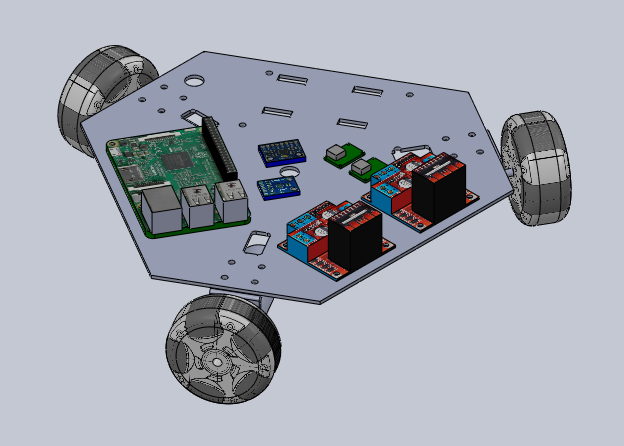
\includegraphics[width = 0.45\textwidth]{imagens/proto01}
  \caption{Chassi projetado. TROCAR A IMAGEM.}
  \label{fig:chassi}
\end{figure}

O custo de aquisição dos componentes relatados pode ser visto detalhado no hyperref[sec:custo]{Apêndice A}. Cabe ressaltar que todos os itens foram comprados em dobro, para realizar a montagem de dois robôs para futuros trabalhos no LAMECC (Laboratório de Mecatrônia e Controle), e que o chassi foi usinado no próprio laboratório com equipamento próprio, sendo computado apenas o custo do material utilizado.


\cite{siegwart2011introduction}, pg 97: sensores.

\section{Desenvolvimento Teórico}
\label{sec:teorico}

%% MODELAGEM:
%PARK: pg 468

Coordenadas de referência na Equação \ref{eq:world_ref} (\cite{siegwart2011introduction}), também utilizado por \cite{ritter2016modelagem}:
\begin{equation}
  \begin{pmatrix}
    x \\
    y \\
    \theta
  \end{pmatrix}
  =
  \begin{pmatrix}
    cos \theta & sen \theta & 0 \\
    -sen\theta & cos \theta & 0 \\
    0          & 0          & 1
  \end{pmatrix}
  \begin{pmatrix}
    x_W \\
    y_W \\
    \theta
  \end{pmatrix}
  \label{eq:world_ref}
\end{equation}

Cinemática direta, para um robô com 3 rodas dispostas em simetria radial em torno do centro da estrutura, é dada pela Equação \ref{eq:dk}. Diversos autores utilizam variações da mesma modelagem (\cite{rojas2006holonomic}, \cite{ritter2016modelagem}, \cite{pin1994new}, entre outros).

\begin{equation}
  \begin{pmatrix}
    v_x \\
    v_y \\
    \omega
  \end{pmatrix}
  =
  \frac{r}{3R}
  \begin{pmatrix}
    -\frac{3R}{\sqrt{3}} & 0   & \frac{3R}{\sqrt{3}} \\
    R                    & -2R & R                   \\
    1                    & 1   & R
  \end{pmatrix}
  \begin{pmatrix}
    \dot{\phi_1} \\
    \dot{\phi_2} \\
    \dot{\phi_3}
  \end{pmatrix}.
  \label{eq:dk}
\end{equation}

Cinemática inversa, obtida realizando a inversão da matriz 3x3, é dada pela Equação \ref{eq:ik}. Nota-se que esta inversão é simplificada no caso do robô com 3 rodas, visto que quando há mais rodas é formada uma matriz 3x$n$, e se deve realizar a pseudo-inversa, conforme demonstrado por \cite{rojas2006holonomic}. Nas equações apresentadas, $r$ é o raio de cada roda e $R$ o raio do robô (a distância do centro da roda ao centro da estrutura do robô).

\begin{equation}
  \begin{pmatrix}
    \dot{\phi_1} \\
    \dot{\phi_2} \\
    \dot{\phi_3}
  \end{pmatrix}.
  =
  \frac{1}{r}
  \begin{pmatrix}
    -\frac{\sqrt(3)}{2} & \frac{1}{2} & R \\
    0                   & -1          & R \\
    \frac{\sqrt(3)}{2}  & \frac{1}{2} & R
  \end{pmatrix}
  \begin{pmatrix}
    v_x \\
    v_y \\
    \omega
  \end{pmatrix}
  \label{eq:ik}
\end{equation}

Como pela classificação de \cite{campion1996structural} um \acrshort{tomr} é caracterizado na categoria (3,0), o modelo cinemático das equações \ref{eq:dk} e \ref{eq:ik} é controlável, estável e descreve a posição, orientação e suas derivadas de forma suficiente. % O modelo cinemático da Equação \ref{eq:dk} também é utilizado por \cite{rojas2006holonomic} e \cite{ritter2016modelagem}.

%% ODOMETRIA:
\cite{samani2007comprehensive}: Descrevem fórmulas para odometria, e dizem que se isso não for muito bom, nem adianta ter um controlador massa. Utilizam três rodas passivas com os encoders, para evitar problemas. Solução a meio enjambrada.

Para se realizar a odometria do robô com uma precisão melhor, \cite{lynch2017modern} ainda fornece as equações relacionadas ao \textbf{body twist} $v_b = (v_{bx}, v_{by}, \omega_b)^T$, que relaciona a velocidade do centro geométrico do robô com as velocidades de cada uma das rodas, que diferem caso o robô realize rotações durante a translação. Tal relação é dada pela Equação \ref{eq:twist}.

\begin{equation}
  v_b = No-entendi-nada.
  \label{eq:twist}
\end{equation}

Modelagens dinâmicas também podem ser utilizadas, relacionando o comportamento do robô não às velocidades das suas rodas, mas sim ao torque aplicado a cada uma pelos motores. No entanto, no caso do \acrshort{tomr}, se podem utilizar as velocidades das rodas como entradas, desde que haja um \emph{loop} de controle que garanta tais velocidades durante o acionamento (CITAR AS NOTAS DE AULA DO WALTER??? control.pdf).

%% PLANEJAMENTO DE TRAJETÓRIA:
\cite{lynch2017modern}, capítulo 9.

%% CONTROLE:
\cite{rojas2006holonomic}: Sugerem que utilizar um controlador para cada roda é melhor do que para cada grau de liberdade. No nosso caso, é tranquilo pois temos apenas 3 rodas, mantendo o mesmo número de controladores. Devido à realimentação externa lenta, utilizam um preditor no robô. Não entram em detalhes.
motores:
https://www.banggood.com/6V-210RPM-Encoder-Motor-DC-Gear-Motor-with-Mounting-Bracket-and-Wheel-p-1044064.html?p=970719369296201312SG

Given a desired trajectory q d (t), we can adopt the feedforward plus proportional feedback linear controller (11.1) of Chapter 11 to track the trajectory: \cite{lynch2017modern}

\cite{samani2007comprehensive}: Definir os coeficientes dos PIDs é uma novela, pois devemos levar em consideração parâmetros que possuem muita variação, como o coeficiente de atrito do solo, características das baterias, entre outros. Controle deles é bem legal.
%q̇ com (t) = q̇ d (t) + K p ( q̇ d (t) − q(t)),
%(13.11)
%where K p ∈ R 3×3 is positive definite and q(t) is an estimate of the actual con-
%figuration derived from sensors. Then q̇ com (t) can be converted to commanded
%wheel driving velocities u com (t) using Equation (13.7).


%: seguimento de trajetória: malha aberta (3.6.1); Feedback (3.6.2) do livro: It is very similar to the controllers presented in [39, 100]. Others can be found in [8, 52, 53, 137]. Controle com uma matriz de ganhos K para o espaço de estados. Estável e tal. Comentam sobre camadas: planejamento -> decisão -> controlador em tempo real -> hardware.



\cite{siegwart2011introduction}: 5.6.3.1 Introduction to Kalman filter theory

%A \textbf{modelagem cinemática} do \acrshort{tomr}, conforme desenvolvida por \cite{campion1996structural} e na forma utilizada por \cite{samani2007comprehensive}, é dada por
%\begin{equation}
%  \begin{pmatrix}
%    \dot{\phi_1} \\
%    \dot{\phi_2} \\
%    \dot{\phi_3}
%  \end{pmatrix}.
%  =
%  \frac{1}{r}
%  \begin{pmatrix}
%    -sen(\theta)               & cos(\theta)                & R \\
%    -sen(\frac{\pi}{3}-\theta) & -cos(\frac{\pi}{3}-\theta) & R \\
%    sen(\frac{\pi}{3}+\theta)  & -cos(\frac{\pi}{3}+\theta) & R
%  \end{pmatrix}
%  \begin{pmatrix}
%    v_x \\
%    v_y \\
%    \omega
%  \end{pmatrix}.
%  \label{eq:pkm}
%\end{equation}


\section{Implementação dos algoritmos}
\label{sec:software}

SEÇÃO EM CONSTRUÇÃO


O \textbf{Raspberry Pi} é um \emph{single board computer}, que utiliza a arquitetura \acrshort{arm} em seu processador, ideal para dispositivos alimentados por baterias por consumir pouca energia e gerar pouco calor. O processador possui quatro núcleos, e um \emph{clock} de 1,2 GHz -- poder computacional equivalente há um computador de mesa comum. O \acrshort{rpi} utiliza um sistema operacional GNU/Linux, e \emph{software} deve ser desenvolvido para ser executado nesta plataforma. Há ainda 40 pinos de \acrshort{gpio} que podem ser utilizados para conectar sensores, atuadores e diversos componentes, e suporte nativo a \acrshort{i2c} (\cite{upton2014raspberry}).


Para a comunicação dos periféricos com este computador, é necessário utilizar algum protocolo de comunicação. O protocolo \textbf{\acrlong{i2c}}, é geralmente utilizado em robôs, csom um grande suporte tanto pela \acrshort{rpi} (\cite{upton2014raspberry}) quanto pelos componentes em geral utilizados (\cite{MPU6050} e a bússola e o arduino se eu usar). Com este protocolo, descrito em \cite{semiconductors2000i2c}, dados podem ser transmitidos a 100 Kbps -- ou 400 Kbps quando utilizado o \emph{fast mode}. São utilizados duas linhas bidirecionais no barramento: SDA para os dados e SCL para os sinais de \emph{clock}. O número de dispositivos conectados ao barramento só depende do limite de capacitância descrito na especificação. Resistores de \emph{pull-up} são necessários para manter a linha em estado lógico alto quando não utilizada, porém estes resistores estão presentes internamente no \emph{Raspberry Pi}, por exemplo.


\section{Avaliação experimental}
\label{sec:experimental}

SEÇÃO EM CONSTRUÇÃO
